\chapter{Vuelo en espiral}

Igual que se ha hecho en el capítulo anterior con el vuelo horizontal, este capítulo pretende abordar el estado del helicóptero durante un vuelo en espiral ascendente con ángulo de asiento de la velocidad $\gamma_T$=5$^\circ$, giro a la derecha y un radio de giro de la trayectoria de 150 m.
Lo primero que salta a la vista en la gráfica \ref{PMVE} es la reducción de la velocidad de avance máxima a la que se puede volar, siendo esta 42.37 m/s, lo que supone una reducción de casi 30 m/s respecto al vuelo horizontal, lo que se debe a la necesidad de invertir una parte importante de la potencia en conseguir una velocidad vertical. Dicha velocidad vertical se ha representado en la gráfica \ref{VzVE}. Al ser el ángulo de asiento de la velocidad constante, la velocidad de ascenso varía de forma casi lineal con la velocidad de avance.

\begin{figure}
	\centering
	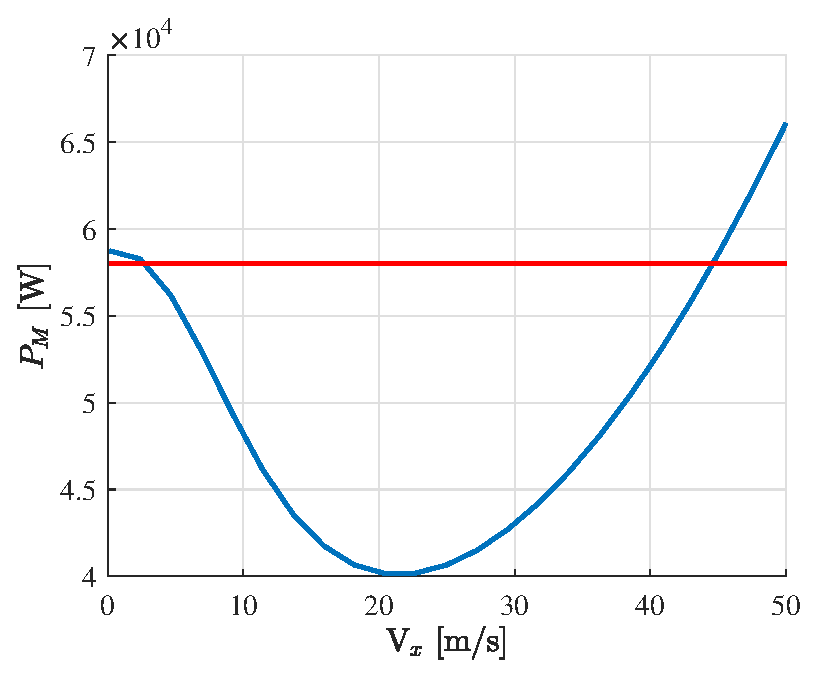
\includegraphics[width=90mm]{graficos/PMVE}
	\caption{Consumo de Potencia de la aeronave en función de la velocidad de avance a nivel del mar para vuelo en espiral ascendente con $\gamma_T$=5$^\circ$, giro a la derecha y radio de la trayectoria 150 m. La línea roja representa el valor de la potencia máxima continua que puede proporcionar el motor.}
	\label{PMVE}
\end{figure}
\begin{figure}
	\centering
	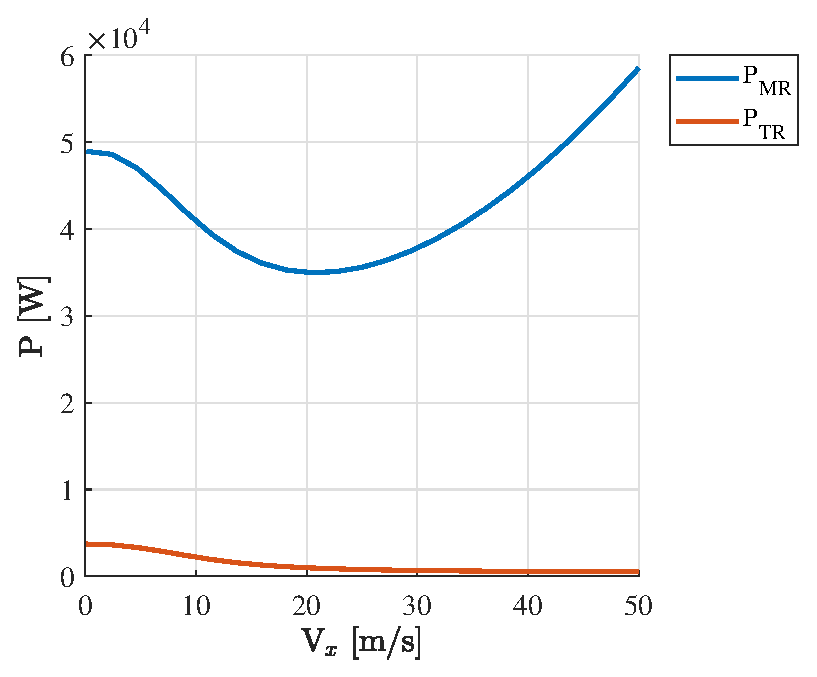
\includegraphics[width=90mm]{graficos/PVE}
	\caption{Consumo de Potencia de los rotores principal y antipar en función de la velocidad de avance a nivel del mar para vuelo en espiral ascendente con $\gamma_T$=5$^\circ$, giro a la derecha y radio de la trayectoria 150 m.}
	\label{PVE}
\end{figure}
\begin{figure}
	\centering
	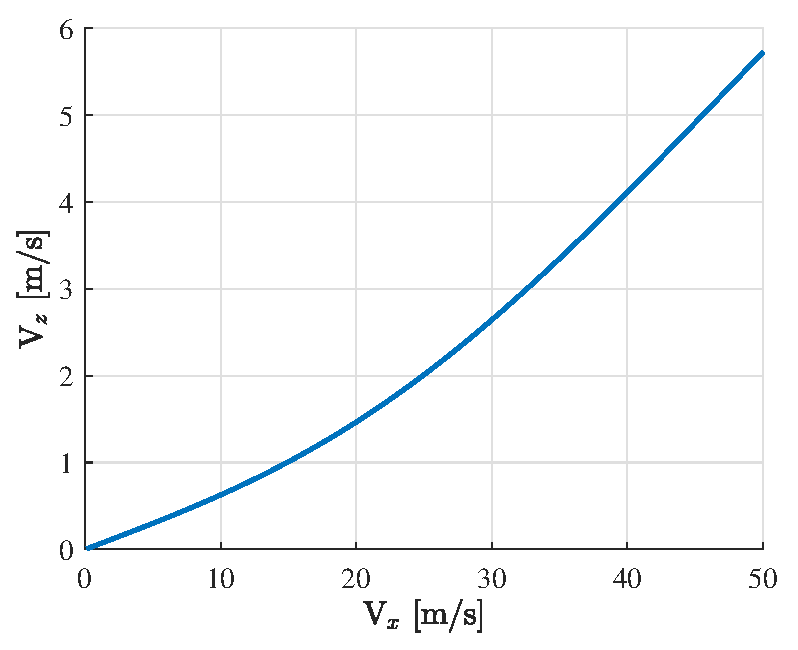
\includegraphics[width=90mm]{graficos/VzVE}
	\caption{Velocidad vertical de la aeronave en función de la velocidad de avance a nivel del mar para vuelo en espiral ascendente con $\gamma_T$=5$^\circ$, giro a la derecha y radio de la trayectoria 150 m.}
	\label{VzVE}
\end{figure}
\begin{figure}
	\centering
	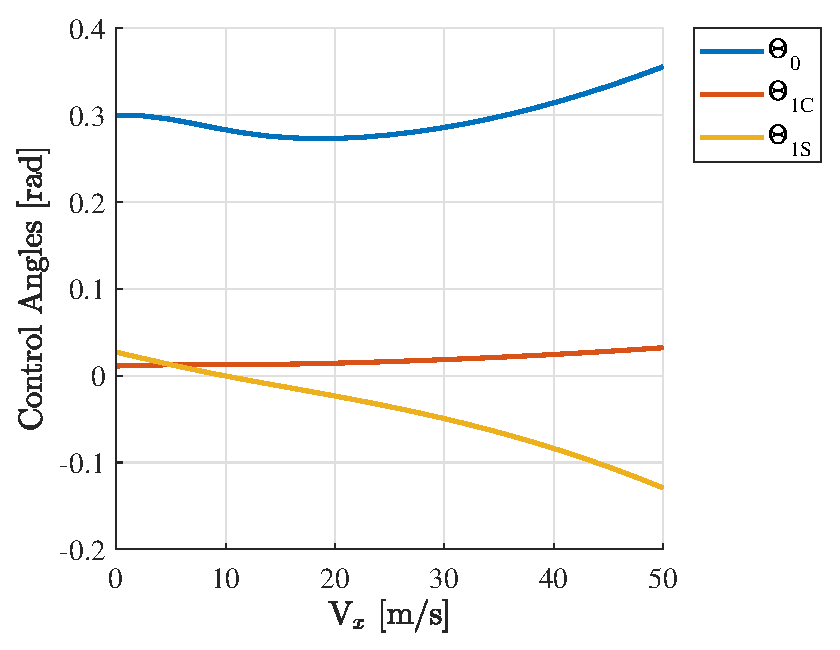
\includegraphics[width=90mm]{graficos/ControlVE}
	\caption{Ángulos de control de la aeronave en función de la velocidad de avance a nivel del mar para vuelo en espiral ascendente con $\gamma_T$=5$^\circ$, giro a la derecha y radio de la trayectoria 150 m.}
	\label{ControlVE}
\end{figure}

Los ángulos de control se han reflejado en gráfica \ref{ControlVE}, y si la comparamos con la gráfica \ref{ControlVH} del vuelo horizontal se puede apreciar que mientras el ángulo de paso cíclico lateral $\theta_{1C}$ sigue una evolución similar, el ángulo de paso colectivo $\theta_0$ aumenta de forma significativa. Esto se debe al incremento de sustentación necesario para poder elevar la aeronave. Por otra parte, se ve como el ángulo de paso longitudinal $\theta_{1S}$ disminuye, ya que la sustentación ha de tener una mayor componente vertical para no solo compensar el peso de la aeronave sino poder elevarla a su vez.

\begin{figure}
	\centering
	\includegraphics[width=90mm]{graficos/EulerVE}
	\caption{Ángulos de Euler de la aeronave en función de la velocidad de avance a nivel del mar para vuelo en espiral ascendente con $\gamma_T$=5$^\circ$, giro a la derecha y radio de la trayectoria 150 m.}
	\label{EulerVE}
\end{figure}

En lo que respecta a los ángulos de Euler, el cambio también resulta lógico. En la gráfica \ref{EulerVH} del capítulo anterior se observa que con la velocidad, apenas cambia el balanceo, mientras que el cabeceo disminuye, pero en la gráfica \ref{EulerVE} par el vuelo en espiral ocurre algo muy distinto.
El ángulo de cabeceo apenas apenas cambia mientras que el ángulo de balanceo aumenta con la velocidad. Si se mantiene constante la curvatura de la espiral, según aumenta la velocidad de avance la aceleración normal necesaria para mantener la trayectoria aumenta, de ahí el origen de ese incremento en el ángulo de balanceo.

\section{Velocidad de ascenso del vuelo}

A diferencia del caso del vuelo horizontal, donde interesaba conocer la autonomía del helicóptero, este tipo de vuelo no será el principal de la aeronave, por lo que en ningún caso el vehículo volará en estas circunstancias durante una fracción relevante de su tiempo de vuelo. Otro parámetro típico que podría calcularse en este tipo de vuelos es el techo de la aeronave, pero como UAV de vigilancia, no interesará que realice vuelos a altitudes muy elevadas pues podría interferir en su misión por no ser las cámaras equipadas capaces de captar imágenes nítidas en esas condiciones.
Sin embargo, si podría resultar interesante observar como varía el vuelo con la velocidad vertical. Para ello se asume que el vehículo vuela con una velocidad absoluta constante de 30 m/s, de esta manera podemos comprobar cual es la velocidad máxima de ascenso que puede alcanzar el helicóptero en el vuelo en espiral.

\begin{figure}
	\centering
	\includegraphics[width=90mm]{graficos/PMVEVz}
	\caption{Consumo de Potencia de la aeronave en función de la velocidad de ascenso a nivel del mar para vuelo en espiral ascendente con velocidad 30m/s, giro a la derecha y radio de la trayectoria 150 m. La línea roja representa el valor de la potencia máxima continua que puede proporcionar el motor.}
	\label{PMVEVz}
\end{figure}
\begin{figure}
	\centering
	\subfigure[Consumo de Potencia de la aeronave en función de la velocidad de ascenso a nivel del mar para vuelo en espiral ascendente con velocidad 20m/s.]{\includegraphics[width=60mm]{graficos/PMVEVz20}}
	\subfigure[Consumo de Potencia de la aeronave en función de la velocidad de ascenso a nivel del mar para vuelo en espiral ascendente con velocidad 10m/s.]{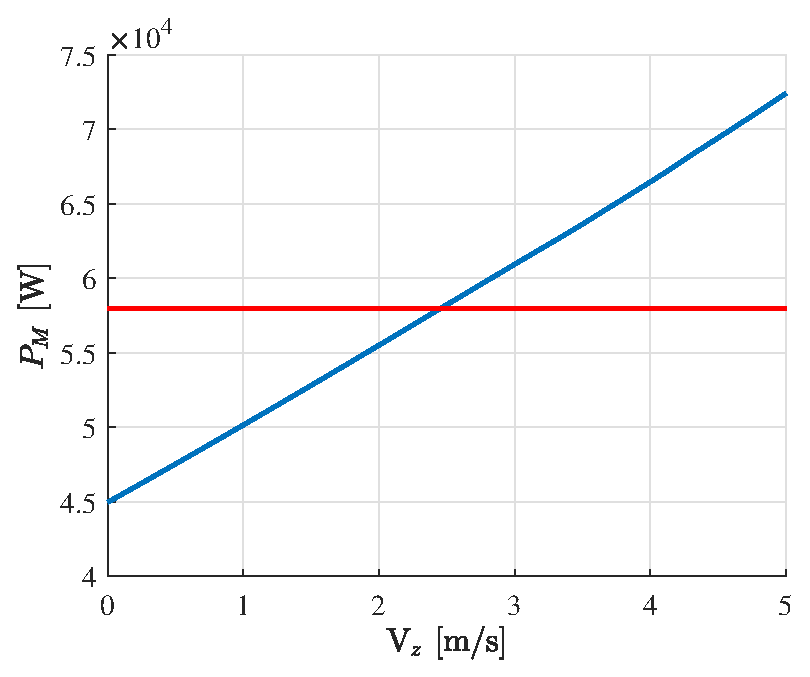
\includegraphics[width=60mm]{graficos/PMVEVz10}}
	\caption{Consumos de Potencia de la aeronave en función de la velocidad de ascenso a nivel del mar para vuelos en espiral ascendente con diferentes velocidades 30m/s giro a la derecha y radio de la trayectoria 150 m. La línea roja representa el valor de la potencia máxima continua que puede proporcionar el motor.}
	\label{PMVEVz2}
\end{figure}
\begin{figure}
	\centering
	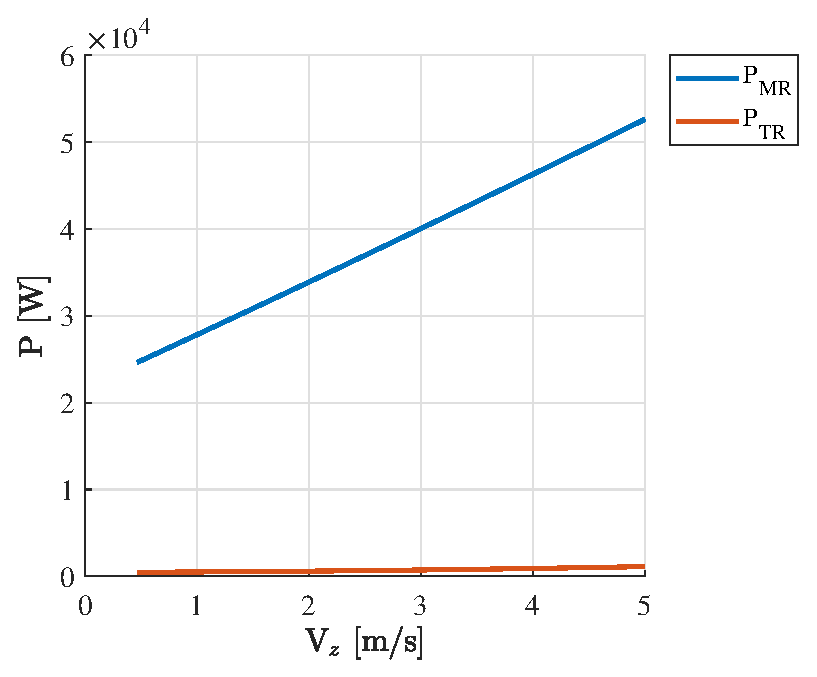
\includegraphics[width=90mm]{graficos/PVEVz}
	\caption{Consumo de Potencia de los rotores principal y antipar en función de la velocidad de ascenso a nivel del mar para vuelo en espiral ascendente con velocidad 30m/s, giro a la derecha y radio de la trayectoria 150 m.}
	\label{PVEVz}
\end{figure}
\begin{figure}
	\centering
	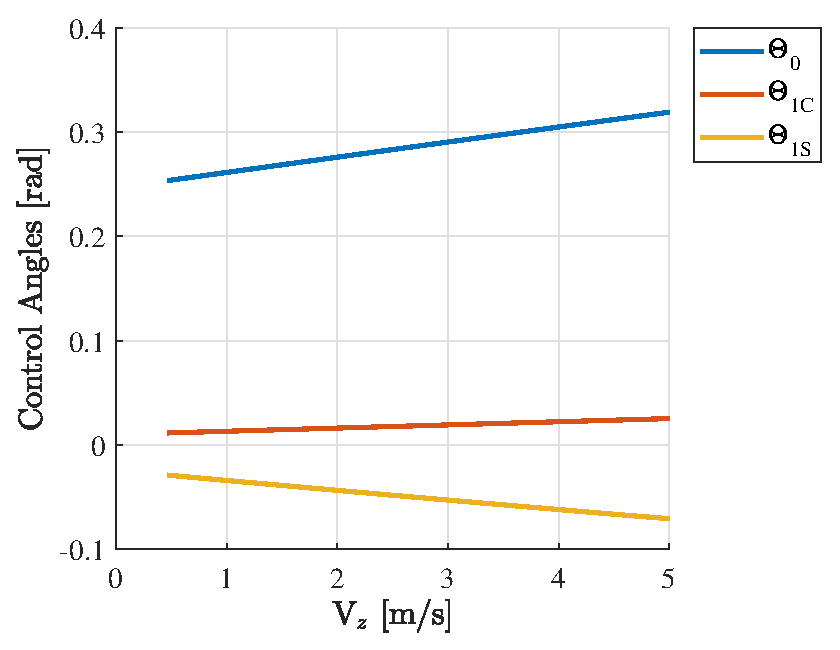
\includegraphics[width=90mm]{graficos/ControlVEVz}
	\caption{Ángulos de control de la aeronave en función de la velocidad de ascenso a nivel del mar para vuelo en espiral ascendente con velocidad 30m/s, giro a la derecha y radio de la trayectoria 150 m.}
	\label{ControlVEVz}
\end{figure}
\begin{figure}
	\centering
	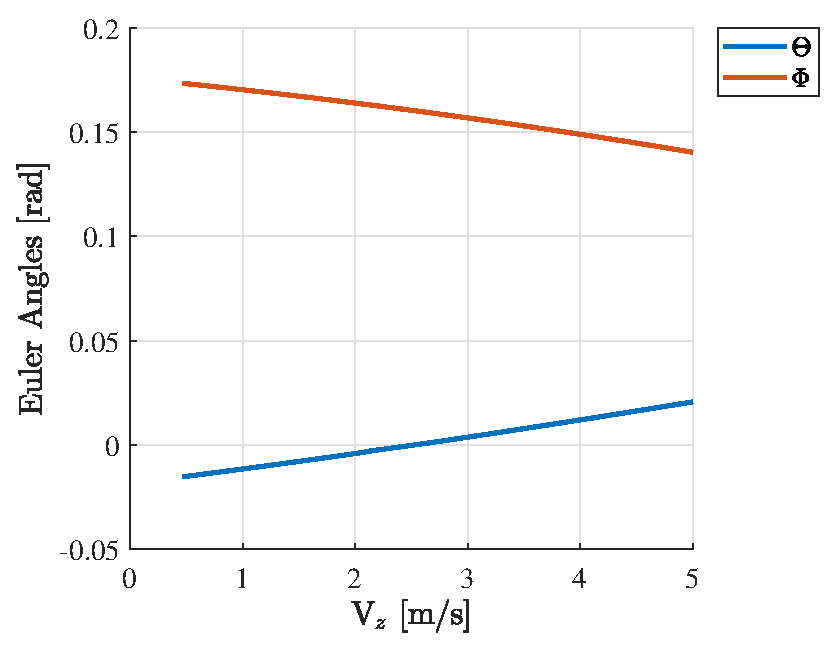
\includegraphics[width=90mm]{graficos/EulerVEVz}
	\caption{Ángulos de Euler de la aeronave en función de la velocidad de ascenso a nivel del mar para vuelo en espiral ascendente con velocidad 30m/s, giro a la derecha y radio de la trayectoria 150 m.}
	\label{EulerVEVz}
\end{figure}

De la gráfica \ref{PMVEVz} se obtiene rápidamente el valor de la velocidad máxima de ascenso disponible en las condiciones de vuelo dadas, 4.71 m/s. Este valor puede ser interesante para calcular el tiempo de recuperación de la trayectoria del vehículo en caso de perder altitud por cualquier motivo.
También existe la posibilidad de volar a menores velocidades; en la gráfica \ref{PMVEVz2} se han representado los mismos resultados para velocidades de vuelo de 20 y 10 m/s. Estos vuelos limitan aún más la velocidad de ascenso máxima, quedando en 4.19 y 2.45 m/s respectivamente. Esto deja claro que una mayor velocidad de vuelo en avance permite también una mayor velocidad de ascenso, pero el cambio en su valor entre las condiciones de vuelo a 20 y 30 m/s, es mucho menor que salto entre las de 10 y 20 m/s, lo que también demuestra que seguir incrementando la velocidad de vuelo no permitirá incrementar la velocidad ascensional de la misma manera.

En la gráfica \ref{PVEVz} se observa que las potencias de ambos rotores se incrementan con la velocidad ascensional, aunque el consumo de potencia del rotor antipar lo hace en menor medida, además de suponer una parte mínima de la potencia consumida.

Las variaciones dadas en los ángulos de control (gráfica \ref{ControlVEVz}) son pequeñas; el paso cíclico longitudinal apenas varía, mientras que el paso colectivo y cíclico lateral lo hacen en mayor medida. Con la velocidad ascensional aumenta el paso colectivo mientras que disminuye el paso ciclico lateral, siendo ambas evoluciones suaves, de un valor absoluto de alrededor de 0.05 rad.

Con los ángulos de Euler pasa algo similar; los cambios son suaves pero apreciables. Con la velocidad de ascenso aumenta el cabeceo mientras que el balanceo disminuye, como se muestra en la gráfica \ref{EulerVEVz}.

\section{Análisis de la carga de pago}

A continuación se exponen los resultados de los análisis realizados a la aeronave en función de la carga de pago embarcada, siendo las cargas posibles las definidas en el capítulo 3.

\subsection*{Integración de las diferentes cargas de pago}

Al igual que se hizo con el caso de vuelo horizontal, se comprabará el efecto de la integración de las diferentes cargas para el caso de vuelo en espiral con $\gamma_T$=5$^\circ$, giro a la derecha y radio de la trayectoria 150 m.

\begin{figure}
	\centering
	\subfigure[Potencia necesaria para el vuelo para diferentes cargas de pago situadas en la proyección del centro de masas de la aeronave en vacío sobre el suelo.]{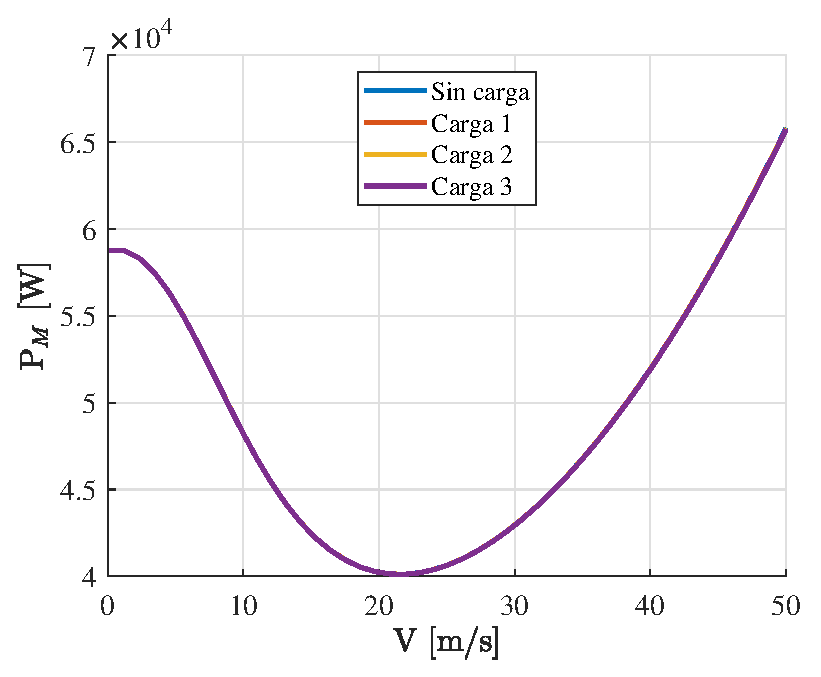
\includegraphics[width=60mm]{graficos/PMVEMPLcdg}}
	\subfigure[Potencia necesaria para el vuelo para diferentes cargas de pago  situadas en $l_x$=1.3 m y $l_y$=-0.2 m.]{\includegraphics[width=60mm]{graficos/PMVEMPLnocdg}}
	\caption{Consumo de Potencia de la aeronave en función de la velocidad de vuelo a nivel del mar para vuelo en espiral con $\gamma_T$=5$^\circ$, giro a la derecha y radio de la trayectoria 150 m para diferentes cargas de pago en posiciones distintas.}
	\label{PMVEMPL}
\end{figure}

De un vistazo a las gráficas \ref{PMVEMPL}, \ref{Theta0VEMPL}, \ref{Theta1CVEMPL}, \ref{Theta1SVEMPL}, \ref{ThetaVEMPL}, \ref{PhiVEMPL} y \ref{Theta0VEraMPL} se puede apreciar que las diferencias para las distintas cargas de pago son similares a las surgidas para el vuelo horizontal del capítulo anterior, por ejemplo, las potencias necesarias para el vuelo apenas varían, siendo ligeramente mayor para la carga 3 a altas velocidades cuando la carga está descentrada.

\begin{figure}
	\centering
	\subfigure[Ángulo de paso colectivo del rotor principal durante el vuelo para diferentes cargas de pago situadas en la proyección del centro de masas de la aeronave en vacío sobre el suelo.]{\includegraphics[width=60mm]{graficos/theta0VEMPLcdg}}
	\subfigure[Ángulo de paso colectivo del rotor principal durante el vuelo para diferentes cargas de pago situadas en $l_x$=1.3 m y $l_y$=-0.2 m.]{\includegraphics[width=60mm]{graficos/theta0VEMPLnocdg}}
	\caption{Ángulos de paso colectivo del rotor principal de la aeronave en función de la velocidad de vuelo a nivel del mar para vuelo en espiral con $\gamma_T$=5$^\circ$, giro a la derecha y radio de la trayectoria 150 m para diferentes cargas de pago en posiciones distintas.}
	\label{Theta0VEMPL}
\end{figure}

En cuanto a los ángulos de paso colectivo del rotor principal, mostrados en la gráfica \ref{Theta0VEMPL}, los cambios son prácticamente iguales, apareciendo los más acusados a altas velocidades para la carga más grande y pesada descentrada. Para cargas centradas o velocidades bajas los cambios son prácticamente inapreciables.

\begin{figure}
	\centering
	\subfigure[Ángulo de paso cíclico longitudinal del rotor principal durante el vuelo para diferentes cargas de pago situadas en la proyección del centro de masas de la aeronave en vacío sobre el suelo.]{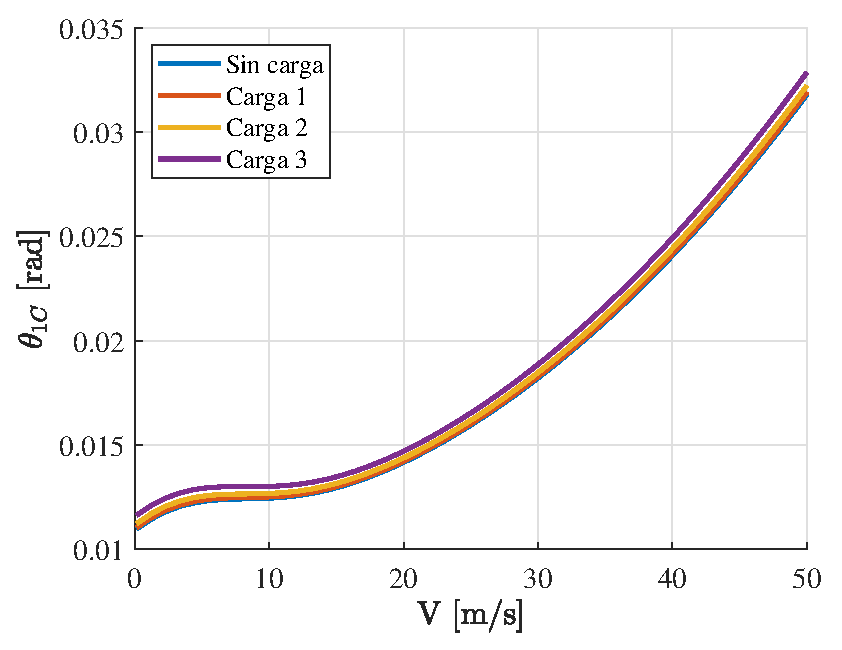
\includegraphics[width=60mm]{graficos/theta1CVEMPLcdg}}
	\subfigure[Ángulo de paso cíclico longitudinal del rotor principal durante el vuelo para diferentes cargas de pago situadas en $l_x$=1.3 m y $l_y$=-0.2 m.]{\includegraphics[width=60mm]{graficos/theta1CVEMPLnocdg}}
	\caption{Ángulos de paso cíclico longitudinal del rotor principal de la aeronave en función de la velocidad de vuelo a nivel del mar para vuelo en espiral con $\gamma_T$=5$^\circ$, giro a la derecha y radio de la trayectoria 150 m para diferentes cargas de pago en posiciones distintas.}
	\label{Theta1CVEMPL}
\end{figure}

Donde se aprecian mayores cambios es en las gráficas \ref{Theta1CVEMPL} y \ref{Theta1SVEMPL}, correspondientes a los ángulos de paso cíclico. Los valores de paso cíclico longitudinal para cargas situadas sobre la proyección del centro de gravedad del helicóptero sufren ligeros incrementos con el tamaño de la carga. Para las cargas descentradas, sin embargo, los valores de paso disminuyen, y estas variaciones son mucho mayores que las dadas en el caso anterior, alcanzando para la carga 3 un valor alrededor de 0.005 rad.

\begin{figure}
	\centering
	\subfigure[Ángulo de paso cíclico lateral del rotor principal durante el vuelo para diferentes cargas de pago situadas en la proyección del centro de masas de la aeronave en vacío sobre el suelo.]{\includegraphics[width=60mm]{graficos/theta1SVEMPLcdg}}
	\subfigure[Ángulo de paso cíclico lateral del rotor principal durante el vuelo para diferentes cargas de pago situadas en $l_x$=1.3 m y $l_y$=-0.2 m.]{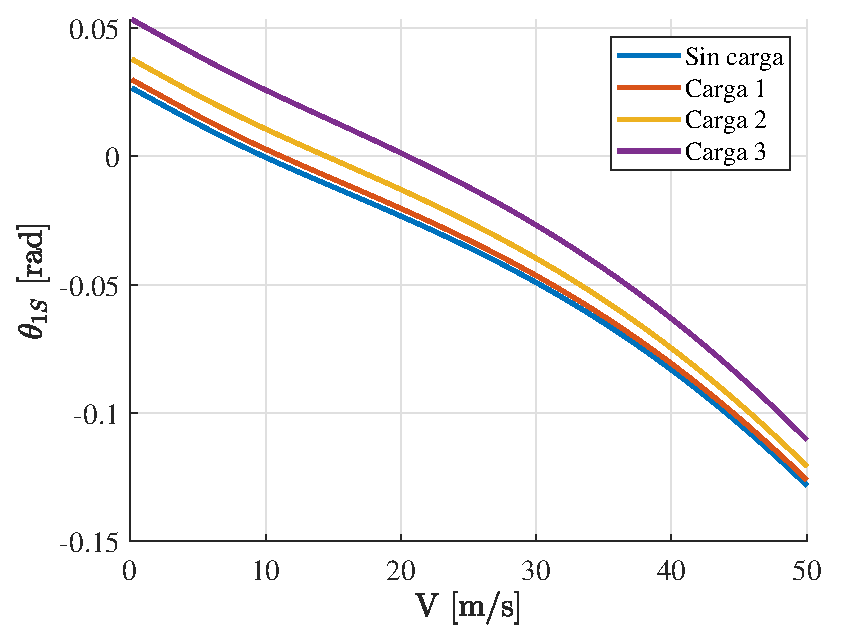
\includegraphics[width=60mm]{graficos/theta1SVEMPLnocdg}}
	\caption{Ángulos de paso cíclico lateral del rotor principal de la aeronave en función de la velocidad de vuelo a nivel del mar para vuelo en espiral con $\gamma_T$=5$^\circ$, giro a la derecha y radio de la trayectoria 150 m para diferentes cargas de pago en posiciones distintas.}
	\label{Theta1SVEMPL}
\end{figure}

El paso cíclico lateral, por su parte, apenas sufre cambios para cargas situadas bajo el centro de masas del vehículo, pero al descentrarlas el paso aumenta ligeramente con la carga. Además, cabe destacar que el incremento del paso dado al cambiar la carga uno por la carga 2 es mucho menor que el dado al cambiar esta por la carga 3, lo que indica que la variación no es lineal.

\begin{figure}
	\centering
	\subfigure[Ángulo de cabeceo de la aeronave durante el vuelo para diferentes cargas de pago situadas en la proyección del centro de masas de la aeronave en vacío sobre el suelo.]{\includegraphics[width=60mm]{graficos/CabVEMPLcdg}}
	\subfigure[Ángulo de cabeceo de la aeronave durante el vuelo para diferentes cargas de pago situadas en $l_x$=1.3 m y $l_y$=-0.2 m.]{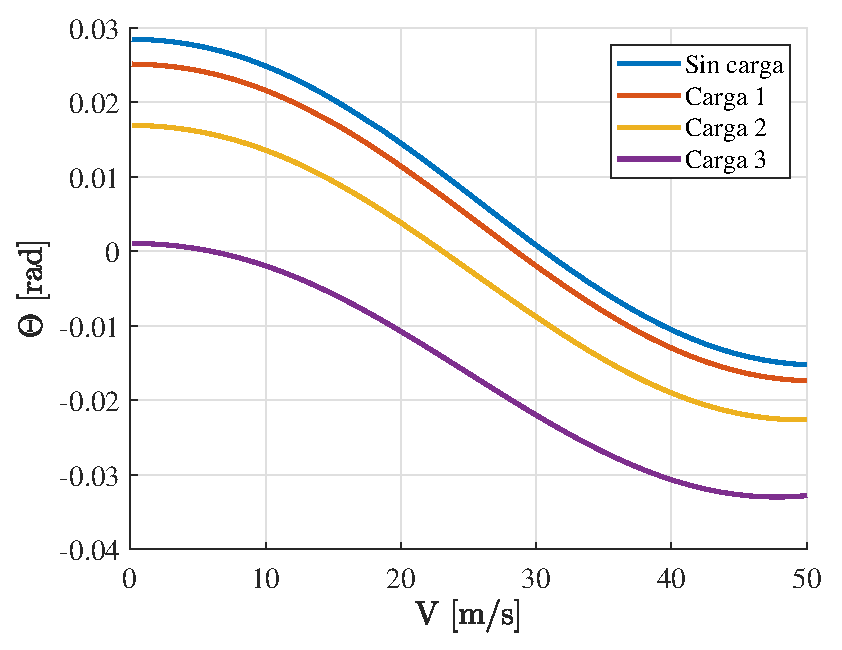
\includegraphics[width=60mm]{graficos/CabVEMPLnocdg}}
	\caption{Ángulos de cabeceo de la aeronave en función de la velocidad de vuelo a nivel del mar para vuelo en espiral con $\gamma_T$=5$^\circ$, giro a la derecha y radio de la trayectoria 150 m para diferentes cargas de pago en posiciones distintas.}
	\label{ThetaVEMPL}
\end{figure}

En la gráfica \ref{ThetaVEMPL} se puede ver la evolución del ángulo de balanceo, que para cargas sobre la proyección del centro de masas del helicóptero, mayores cargas suavizan muy ligeramente las variaciones del mismo con la velocidad, reduciendo su valor absoluto para velocidades muy altas y muy bajas. Al desplazar las cargas, las diferencias se incrementan con el tamaño de la misma, llegando a valores de 0.027 rad para la carga 3 a bajas velocidades, donde son mayores. El aumento de las cargas disminuye el ángulo de cabeceo durante el vuelo, siendo esta evolución de tipo no lineal, al embarcar la carga 2 se disminuye el cabeceo en 0.012 rad, mientras que al cambiar esta por la carga 3, se produce una segunda disminución de 0.015 rad.

\begin{figure}
	\centering
 	\subfigure[Ángulo de balanceo de la aeronave durante el vuelo para diferentes cargas de pago situadas en la proyección del centro de masas de la aeronave en vacío sobre el suelo.]{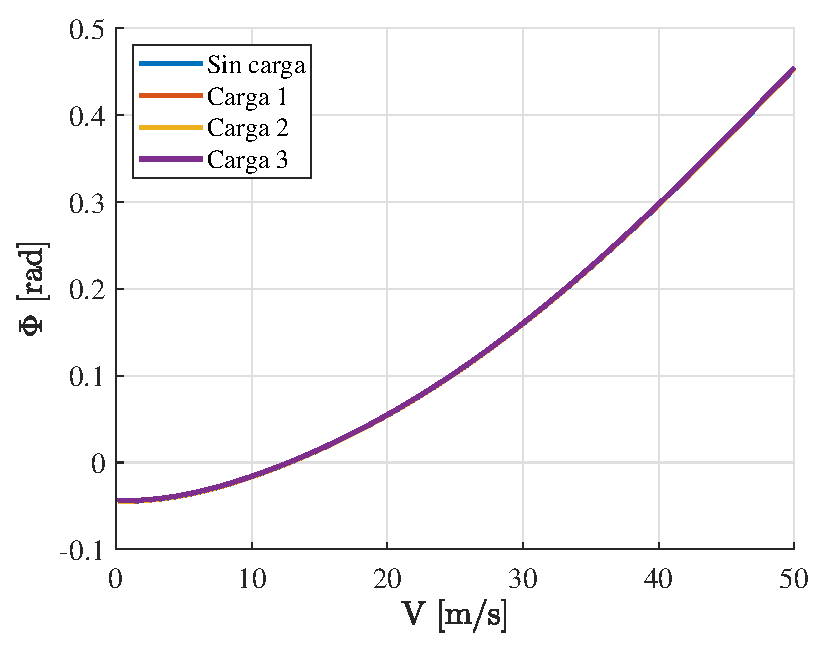
\includegraphics[width=60mm]{graficos/BalanVEMPLcdg}}
	\subfigure[Ángulo de balanceo de la aeronave durante el vuelo para diferentes cargas de pago situadas en $l_x$=1.3 m y $l_y$=-0.2 m.]{\includegraphics[width=60mm]{graficos/BalanVEMPLnocdg}}
	\caption{Ángulos de balanceo de la aeronave en función de la velocidad de vuelo a nivel del mar para vuelo en espiral con $\gamma_T$=5$^\circ$, giro a la derecha y radio de la trayectoria 150 m para diferentes cargas de pago en posiciones distintas.}
	\label{PhiVEMPL}
\end{figure}

El ángulo de balanceo apenas varía con la carga, ni situándola sobre la proyección del centro de masas de la aeronave ni desplazándola. Con la carga desplazada, se puede apreciar en la gráfica \ref{PhiVEMPL} una muy pequeña disminución con la carga, pero esta variación alcanza únicamente valores de 0.0025 rad.

\begin{figure}
	\centering
	\subfigure[Ángulo de paso colectivo del rotor antipar durante el vuelo para diferentes cargas de pago situadas en la proyección del centro de masas de la aeronave en vacío sobre el suelo.]{\includegraphics[width=60mm]{graficos/theta0VEraMPLcdg}}
	\subfigure[Ángulo de paso colectivo del rotor antipar durante el vuelo para diferentes cargas de pago situadas en $l_x$=1.3 m y $l_y$=-0.2 m.]{\includegraphics[width=60mm]{graficos/theta0VEraMPLnocdg}}
	\caption{Ángulos de paso colectivo del rotor antipar de la aeronave en función de la velocidad de vuelo a nivel del mar para vuelo en espiral con $\gamma_T$=5$^\circ$, giro a la derecha y radio de la trayectoria 150 m para diferentes cargas de pago en posiciones distintas.}
	\label{Theta0VEraMPL}
\end{figure}

Por último, la evolución del ángulo de paso colectivo del rotor antipar apenas sufre variaciones con la carga cuando esta se sitúa sobre la proyección del centro de masas del helicóptero. Sin embargo, en la gráfica \ref{Theta0VEraMPL} se puede apreciar que al colocar la carga en la posición indicada, el paso disminuye con la masa de la misma a bajas velocidades, mientras que altas velocidades aumenta. Estas variaciones son máximas a bajas velocidades y alcanzan valores de 0.0025 rad.

\subsection*{Análisis de los parámetros de vuelo con la posición de la carga de pago}

Resulta interesante saber como afecta la posición de la carga de pago a los parámetros de vuelo dadas unas condiciones de vuelo concretas, para poder optimizar el montaje de los equipos según las necesidades de la misión.

\begin{figure}
	\centering
	\subfigure[Potencia necesaria para el vuelo en función de la posición relativa a $O_f$ de la carga 2 para una velocidad de vuelo de 5 m/s.]{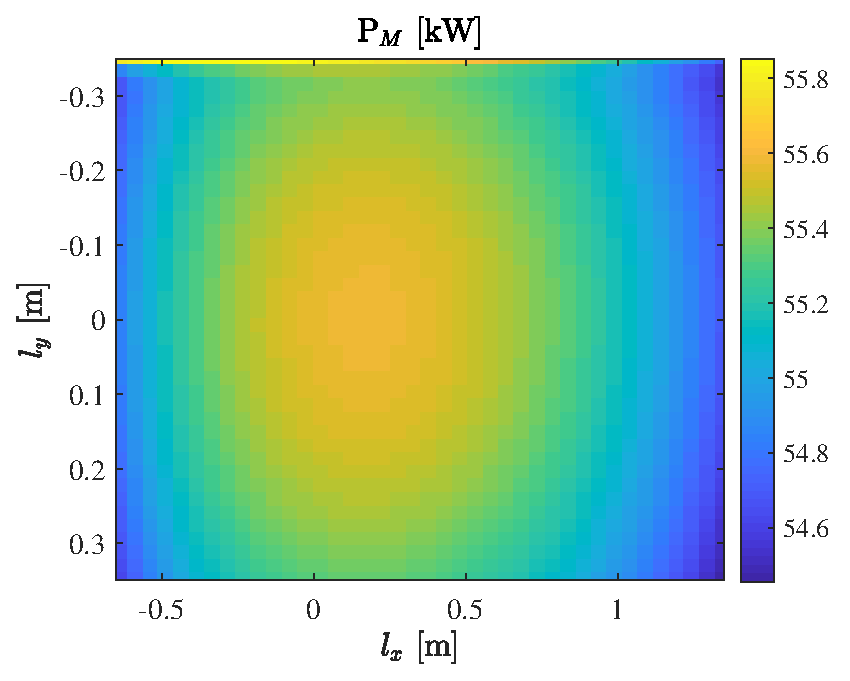
\includegraphics[width=60mm]{graficos/PMVE2lxy5ms}}
	\subfigure[Potencia necesaria para el vuelo en función de la posición relativa a $O_f$ de la carga 2 para una velocidad de vuelo de 35 m/s.]{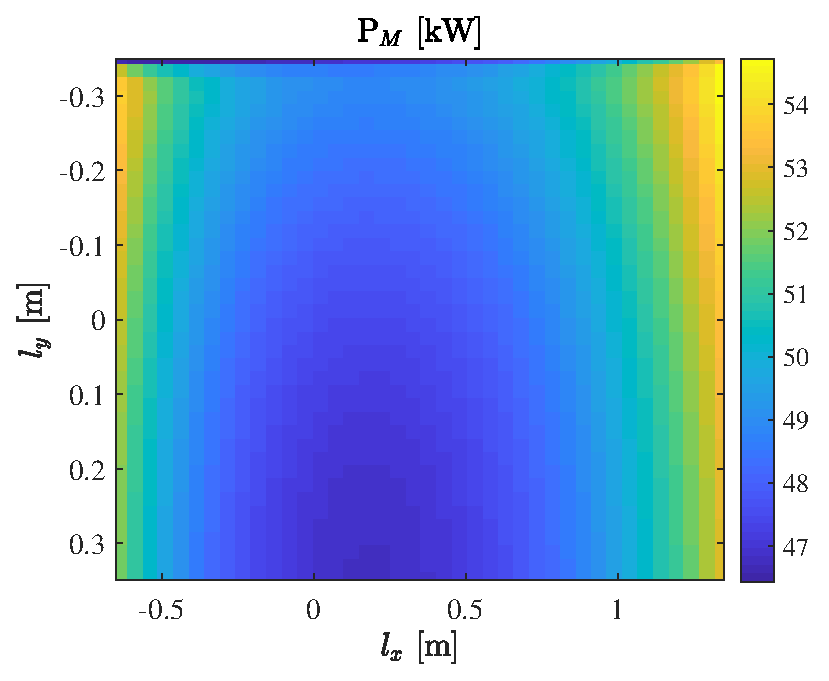
\includegraphics[width=60mm]{graficos/PMVE2lxy35ms}}
	\caption{Consumo de Potencia de la aeronave en función de la posición relativa a $O_f$ de la carga 2 para vuelo en espiral con $\gamma_T$=5$^\circ$, giro a la derecha y radio de la trayectoria 150 m embarcando la carga 2 en posiciones distintas.}
	\label{PMVE2lxy}
\end{figure}
\begin{figure}
	\centering
	\subfigure[Potencia necesaria para el vuelo en función de la posición relativa a $O_f$ de la carga 3 para una velocidad de vuelo de 5 m/s.]{\includegraphics[width=60mm]{graficos/PMVE3lxy5ms}}
	\subfigure[Potencia necesaria para el vuelo en función de la posición relativa a $O_f$ de la carga 3 para una velocidad de vuelo de 35 m/s.]{\includegraphics[width=60mm]{graficos/PMVE3lxy35ms}}
	\caption{Consumo de Potencia de la aeronave en función de la posición relativa a $O_f$ de la carga 3 para vuelo en espiral con $\gamma_T$=5$^\circ$, giro a la derecha y radio de la trayectoria 150 m embarcando la carga 3 en posiciones distintas.}
	\label{PMVE3lxy}
\end{figure}

Si se analiza primero el consumo de potencia para el vuelo, representado en las gráficas \ref{PMVE2lxy} y \ref{PMVE3lxy}, resulta llamativo el resultado para velocidades bajas. Estos indican que el punto mas desfavorable para la colocación de la carga es la proyección del centro de masas de la aeronave sobre el suelo del fuselaje, independientemente de la carga. 
Para altas velocidades este comportamiento cambia, siendo el punto más favorable el centrado longitudinalmente con el centro de masas pero desviado lateralmente hacia la parte derecha del fuselaje.

Cabe destacar también que a mayor carga, los efectos de la posición de la misma sobre la potencia necesaria son mayores también a altas velocidades.

\begin{figure}
	\centering
	\subfigure[Ángulo de paso colectivo del rotor principal en función de la posición relativa a $O_f$ de la carga 2 para una velocidad de vuelo de 5 m/s.]{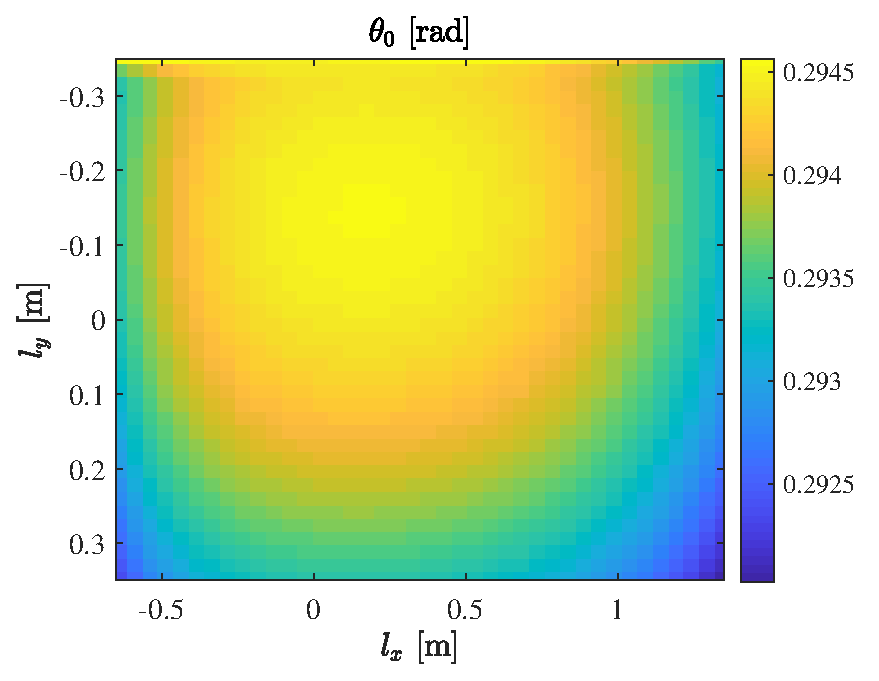
\includegraphics[width=60mm]{graficos/theta0VE2lxy5ms}}
	\subfigure[Ángulo de paso colectivo del rotor principal en función de la posición relativa a $O_f$ de la carga 2 para una velocidad de vuelo de 35 m/s.]{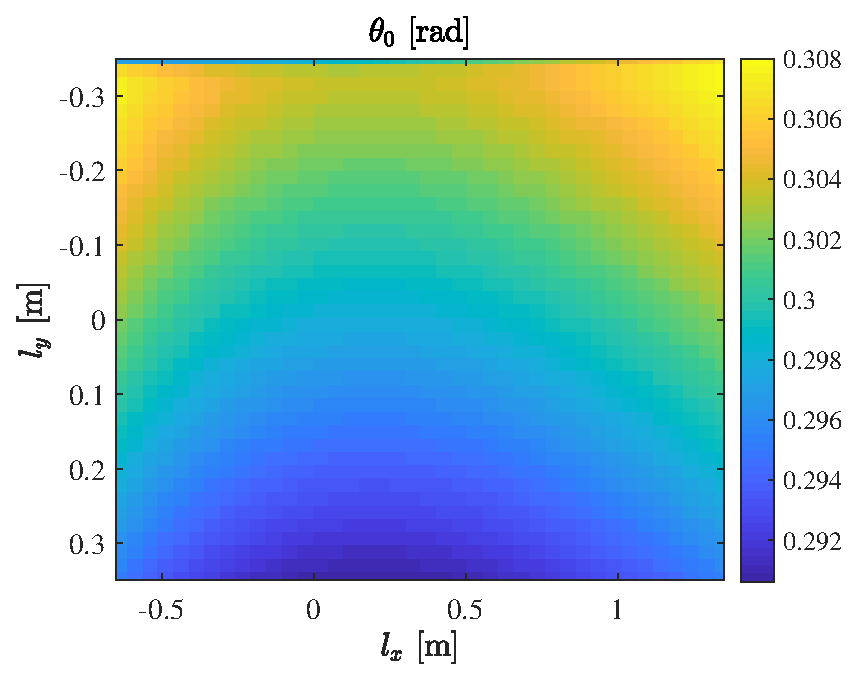
\includegraphics[width=60mm]{graficos/theta0VE2lxy35ms}}
	\caption{Ángulo de paso colectivo del rotor principal en función de la posición relativa a $O_f$ de la carga 2 para vuelo en espiral con $\gamma_T$=5$^\circ$, giro a la derecha y radio de la trayectoria 150 m embarcando la carga 2 en posiciones distintas.}
	\label{theta0VE2lxy}
\end{figure}
\begin{figure}
	\centering
	\subfigure[Ángulo de paso colectivo del rotor principal en función de la posición relativa a $O_f$ de la carga 3 para una velocidad de vuelo de 5 m/s.]{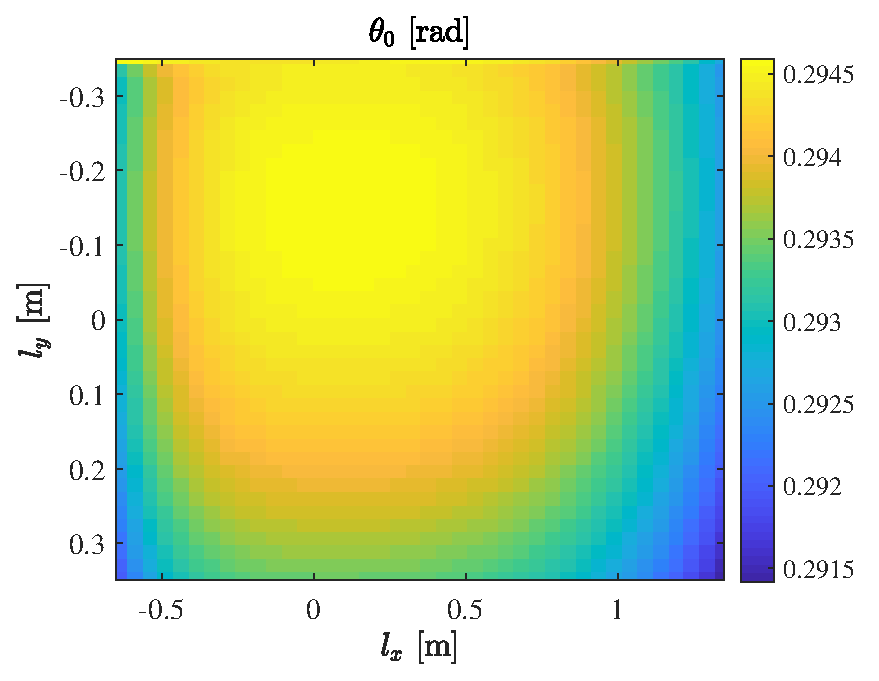
\includegraphics[width=60mm]{graficos/theta0VE3lxy5ms}}
	\subfigure[Ángulo de paso colectivo del rotor principal en función de la posición relativa a $O_f$ de la carga 3 para una velocidad de vuelo de 35 m/s.]{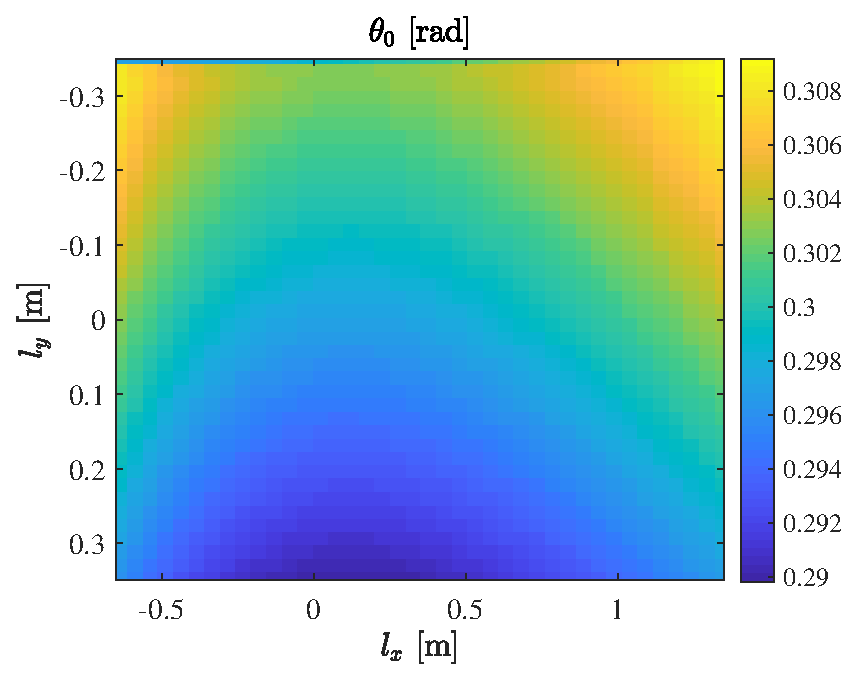
\includegraphics[width=60mm]{graficos/theta0VE3lxy35ms}}
	\caption{Ángulo de paso colectivo del rotor principal en función de la posición relativa a $O_f$ de la carga 3 para vuelo en espiral con $\gamma_T$=5$^\circ$, giro a la derecha y radio de la trayectoria 150 m embarcando la carga 3 en posiciones distintas.}
	\label{theta0VE3lxy}
\end{figure}

Si se observan las gráficas \ref{theta0VE2lxy} y \ref{theta0VE3lxy}, se puede observar que el ángulo de paso colectivo a bajas velocidades se incrementa al centrar longitudinalmente la carga sobre la proyección del centro de masas del vehículo. Lateralmente, existe un máximo del paso para valores de $l_y$ próximos a -0.15 m. Estas afirmaciones se cumplen para ambas cargas, siendo para el caso de la carga 3 los valores del paso ligeramente mayores en un mayor rango de posiciones.
Para altas velocidades, el centrado longitudinal antes mencionado contribuye a la reducción del valor de paso, al igual que el desplazamiento lateral hacia la derecha de la carga.

\begin{figure}
	\centering
	\subfigure[Ángulo de paso cíclico longitudinal en función de la posición relativa a $O_f$ de la carga 2 para una velocidad de vuelo de 5 m/s.]{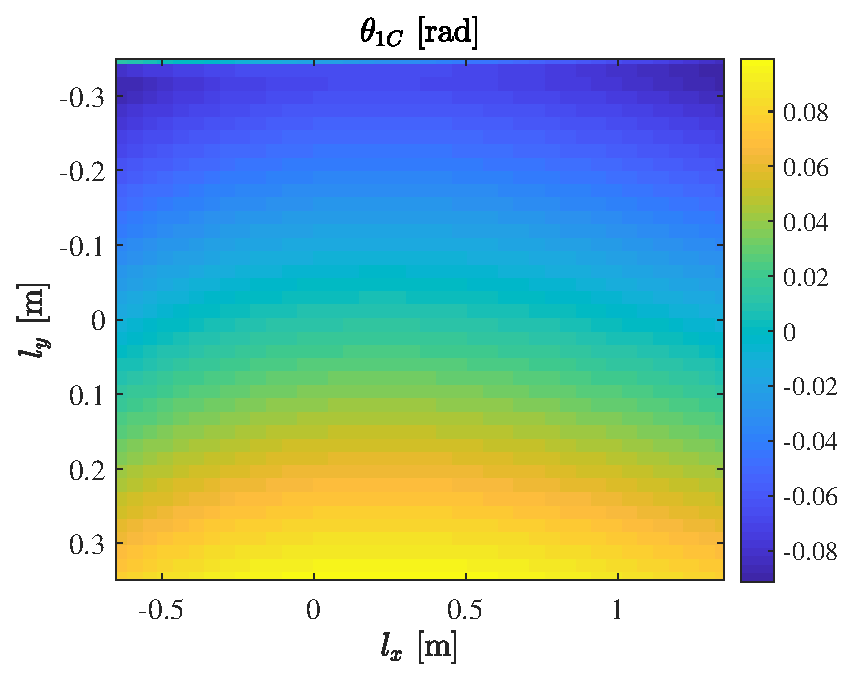
\includegraphics[width=60mm]{graficos/theta1CVE2lxy5ms}}
	\subfigure[Ángulo de paso cíclico longitudinal en función de la posición relativa a $O_f$ de la carga 2 para una velocidad de vuelo de 35 m/s.]{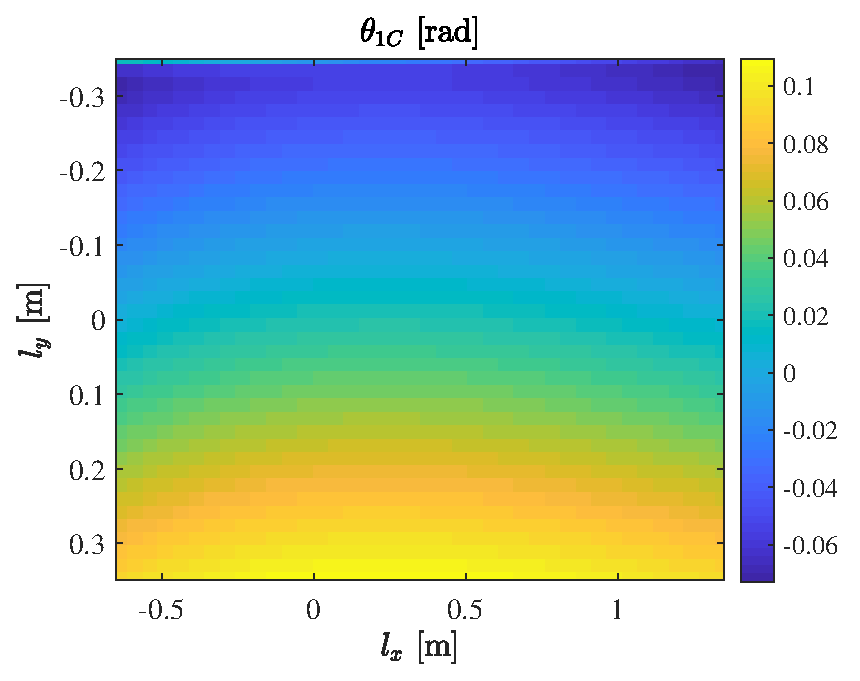
\includegraphics[width=60mm]{graficos/theta1CVE2lxy35ms}}
	\caption{Ángulo de paso cíclico longitudinal en función de la posición relativa a $O_f$ de la carga 2 para vuelo en espiral con $\gamma_T$=5$^\circ$, giro a la derecha y radio de la trayectoria 150 m embarcando la carga 2 en posiciones distintas.}
	\label{theta1CVE2lxy}
\end{figure}
\begin{figure}
	\centering
	\subfigure[Ángulo de paso cíclico longitudinal en función de la posición relativa a $O_f$ de la carga 3 para una velocidad de vuelo de 5 m/s.]{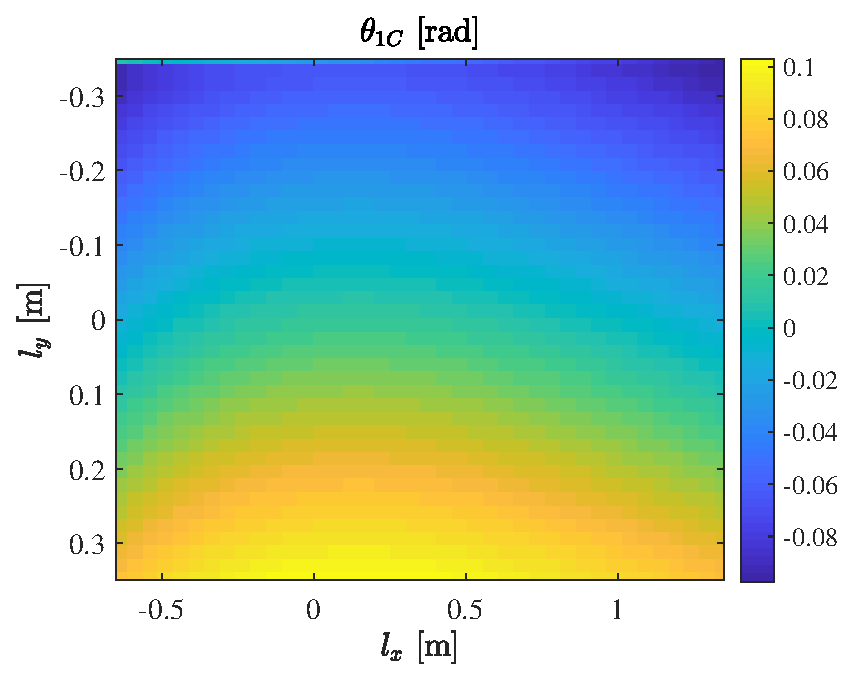
\includegraphics[width=60mm]{graficos/theta1CVE3lxy5ms}}
	\subfigure[Ángulo de paso cíclico longitudinal en función de la posición relativa a $O_f$ de la carga 3 para una velocidad de vuelo de 35 m/s.]{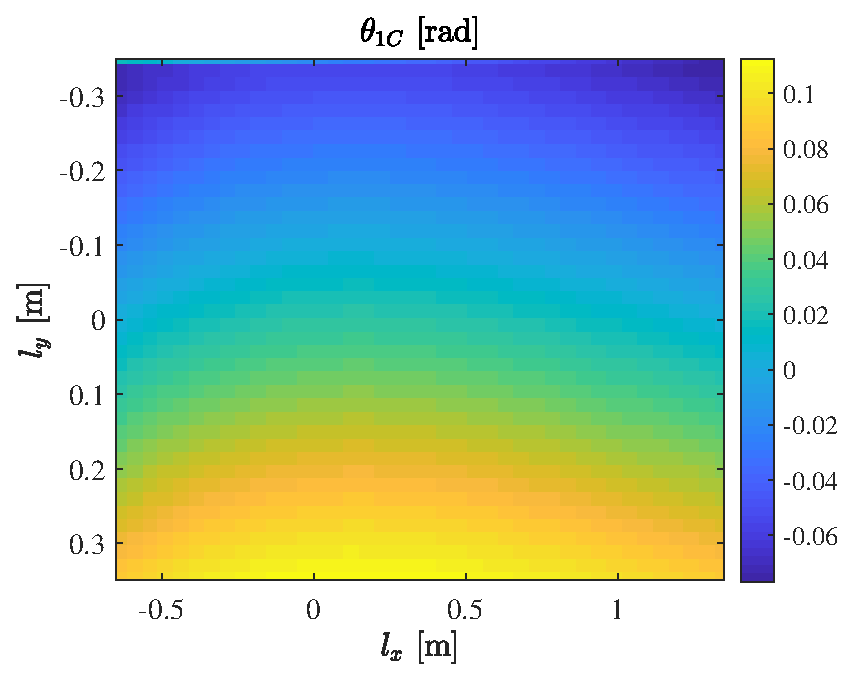
\includegraphics[width=60mm]{graficos/theta1CVE3lxy35ms}}
	\caption{Ángulo de paso cíclico longitudinal en función de la posición relativa a $O_f$ de la carga 3 para vuelo en espiral con $\gamma_T$=5$^\circ$, giro a la derecha y radio de la trayectoria 150 m embarcando la carga 3 en posiciones distintas.}
	\label{theta1CVE3lxy}
\end{figure}

La variación del paso cíclico longitudinal con la posición de la carga es independiente de la velocidad de vuelo; en las gráficas \ref{theta1CVE2lxy} y \ref{theta1CVE3lxy} se observa que los valores del paso son máximos para la misma posición de la carga que permitía alcanzar el mínimo del paso colectivo, centrada longitudinalmente y desplazada a la derecha del fuselaje. En este caso el tamaño de la carga apenas influye.

Con el ángulo de paso cíclico lateral, representado en las gráfica \ref{theta1SVE2lxy} y \ref{theta1SVE3lxy}, se repite el caso del paso cíclico longitudinal, el efecto del tamaño de la carga o la velocidad apenas afectan al efecto de la posición de la misma.
Se puede observar que los valores máximos del paso se dan para posiciones extremas en el sentido longitudinal, mientras que el desplazamiento lateral de la carga no supone una variación muy grande del mismo, reduciéndose ligeramente al desplazar la carga hacia la izquierda del fuselaje.

\begin{figure}
	\centering
	\subfigure[Ángulo de paso cíclico lateral en función de la posición relativa a $O_f$ de la carga 2 para una velocidad de vuelo de 5 m/s.]{\includegraphics[width=60mm]{graficos/theta1SVE2lxy5ms}}
	\subfigure[Ángulo de paso cíclico lateral en función de la posición relativa a $O_f$ de la carga 2 para una velocidad de vuelo de 35 m/s.]{\includegraphics[width=60mm]{graficos/theta1SVE2lxy35ms}}
	\caption{Ángulo de paso cíclico lateral en función de la posición relativa a $O_f$ de la carga 2 para vuelo en espiral con $\gamma_T$=5$^\circ$, giro a la derecha y radio de la trayectoria 150 m embarcando la carga 2 en posiciones distintas.}
	\label{theta1SVE2lxy}
\end{figure}
\begin{figure}
	\centering
	\subfigure[Ángulo de paso cíclico lateral en función de la posición relativa a $O_f$ de la carga 3 para una velocidad de vuelo de 5 m/s.]{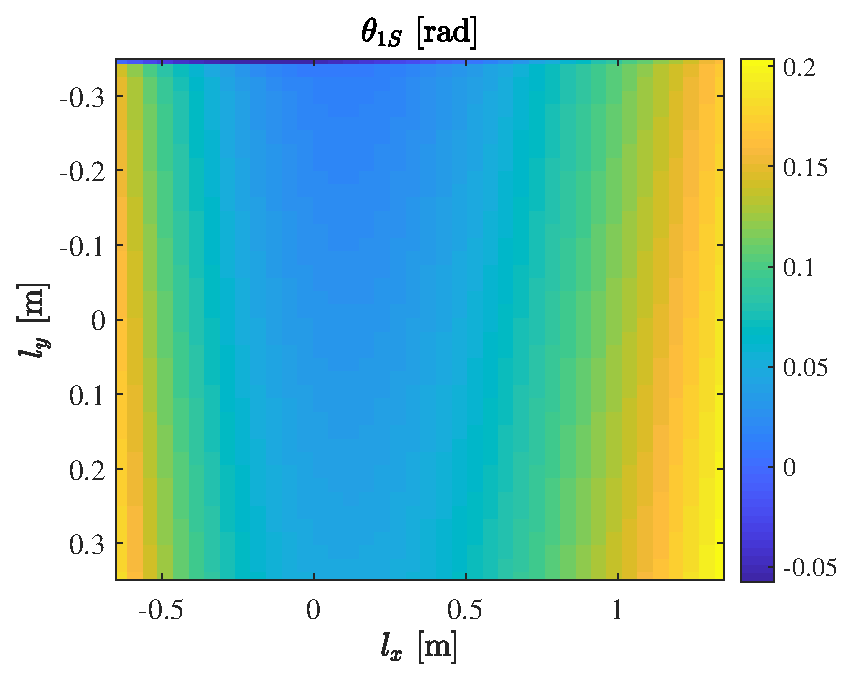
\includegraphics[width=60mm]{graficos/theta1SVE3lxy5ms}}
	\subfigure[Ángulo de paso cíclico lateral en función de la posición relativa a $O_f$ de la carga 3 para una velocidad de vuelo de 35 m/s.]{\includegraphics[width=60mm]{graficos/theta1SVE3lxy35ms}}
	\caption{Ángulo de paso cíclico lateral en función de la posición relativa a $O_f$ de la carga 3 para vuelo en espiral con $\gamma_T$=5$^\circ$, giro a la derecha y radio de la trayectoria 150 m embarcando la carga 3 en posiciones distintas.}
	\label{theta1SVE3lxy}
\end{figure}
\begin{figure}
	\centering
	\subfigure[Ángulo de cabeceo de la aeronave en función de la posición relativa a $O_f$ de la carga 2 para una velocidad de vuelo de 5 m/s.]{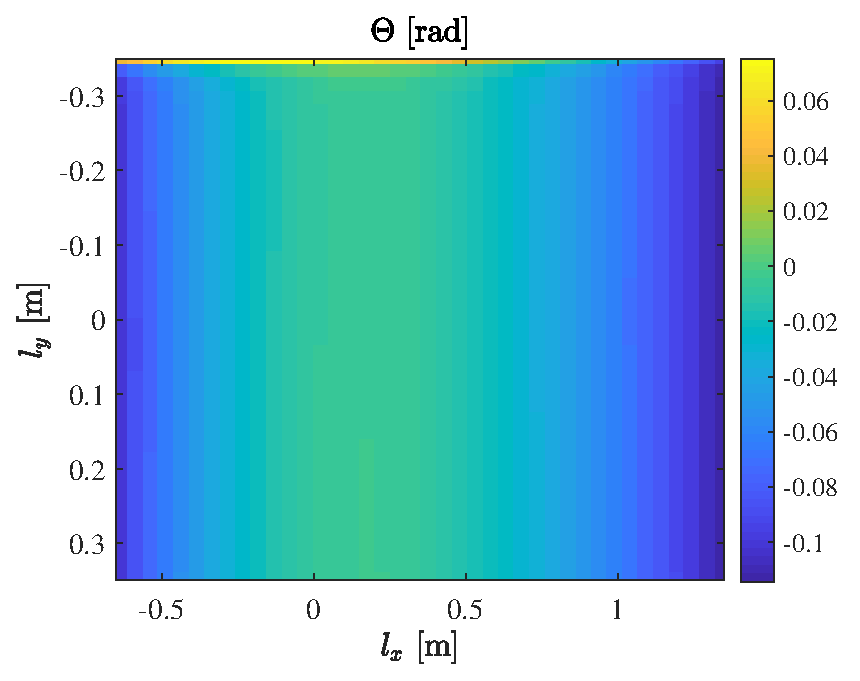
\includegraphics[width=60mm]{graficos/CabVE2lxy5ms}}
	\subfigure[Ángulo de cabeceo de la aeronave en función de la posición relativa a $O_f$ de la carga 2 para una velocidad de vuelo de 35 m/s.]{\includegraphics[width=60mm]{graficos/CabVE2lxy35ms}}
	\caption{Ángulo de cabeceo de la aeronave en función de la posición relativa a $O_f$ de la carga 2 para vuelo en espiral con $\gamma_T$=5$^\circ$, giro a la derecha y radio de la trayectoria 150 m embarcando la carga 2 en posiciones distintas.}
	\label{CabVE2lxy}
\end{figure}
\begin{figure}
	\centering
	\subfigure[Ángulo de cabeceo de la aeronave en función de la posición relativa a $O_f$ de la carga 3 para una velocidad de vuelo de 5 m/s.]{\includegraphics[width=60mm]{graficos/CabVE3lxy5ms}}
	\subfigure[Ángulo de cabeceo de la aeronave en función de la posición relativa a $O_f$ de la carga 3 para una velocidad de vuelo de 35 m/s.]{\includegraphics[width=60mm]{graficos/CabVE3lxy35ms}}
	\caption{Ángulo de cabeceo de la aeronave en función de la posición relativa a $O_f$ de la carga 3 para vuelo en espiral con $\gamma_T$=5$^\circ$, giro a la derecha y radio de la trayectoria 150 m embarcando la carga 3 en posiciones distintas.}
	\label{CabVE3lxy}
\end{figure}
\begin{figure}
	\centering
	\subfigure[Ángulo de balanceo de la aeronave en función de la posición relativa a $O_f$ de la carga 2 para una velocidad de vuelo de 5 m/s.]{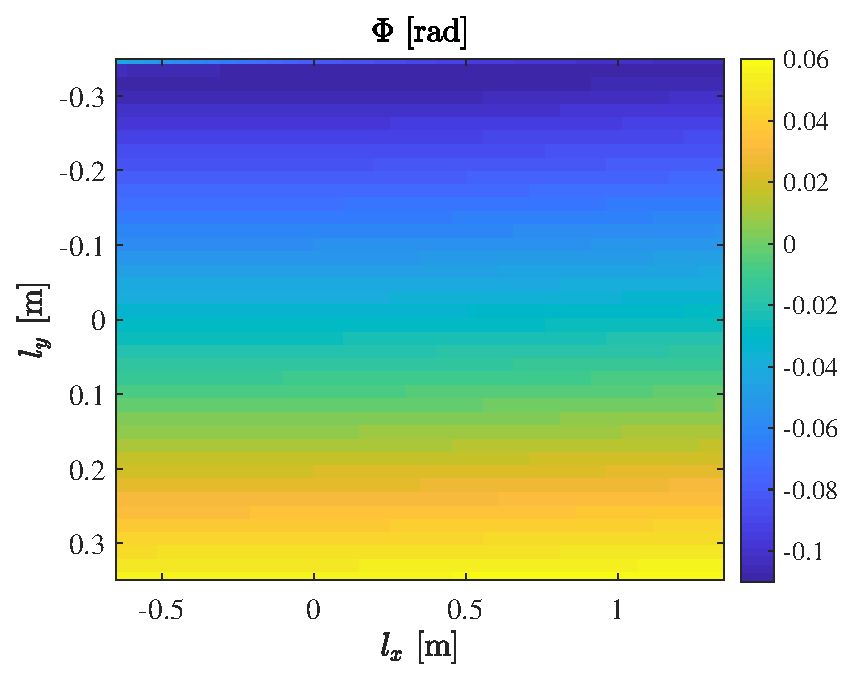
\includegraphics[width=60mm]{graficos/BalanVE2lxy5ms}}
	\subfigure[Ángulo de balanceo de la aeronave en función de la posición relativa a $O_f$ de la carga 2 para una velocidad de vuelo de 35 m/s.]{\includegraphics[width=60mm]{graficos/BalanVE2lxy35ms}}
	\caption{Ángulo de balanceo de la aeronave en función de la posición relativa a $O_f$ de la carga 2 para vuelo en espiral con $\gamma_T$=5$^\circ$, giro a la derecha y radio de la trayectoria 150 m embarcando la carga 2 en posiciones distintas.}
	\label{BalanVE2lxy}
\end{figure}
\begin{figure}
	\centering
	\subfigure[Ángulo de balanceo de la aeronave en función de la posición relativa a $O_f$ de la carga 3 para una velocidad de vuelo de 5 m/s.]{\includegraphics[width=60mm]{graficos/BalanVE3lxy5ms}}
	\subfigure[Ángulo de balanceo de la aeronave en función de la posición relativa a $O_f$ de la carga 3 para una velocidad de vuelo de 35 m/s.]{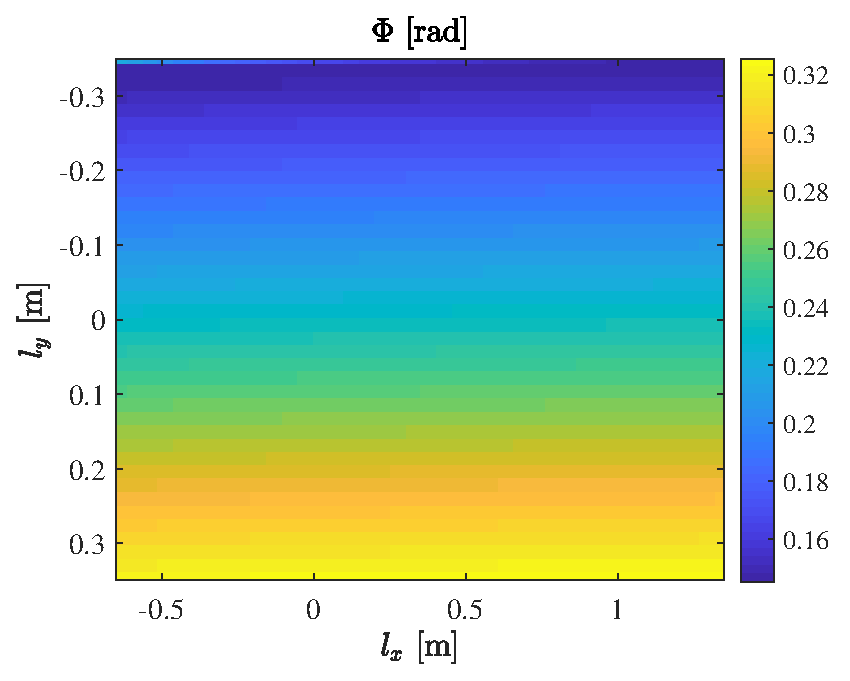
\includegraphics[width=60mm]{graficos/BalanVE3lxy35ms}}
	\caption{Ángulo de balanceo de la aeronave en función de la posición relativa a $O_f$ de la carga 3 para vuelo en espiral con $\gamma_T$=5$^\circ$, giro a la derecha y radio de la trayectoria 150 m embarcando la carga 3 en posiciones distintas.}
	\label{BalanVE3lxy}
\end{figure}

Al observar las gráficas \ref{CabVE2lxy}, \ref{CabVE3lxy}, \ref{BalanVE2lxy} y \ref{BalanVE3lxy}, correspondientes a los ángulos de Euler de la aeronave, se llega a la conclusión de que el ángulo de cabeceo no se ve afectado por la posición lateral de la carga, igual que el ángulo de balanceo no se ve afectado por la posición longitudinal de la misma.
En cuanto al ángulo de cabeceo, sus valores máximos se obtienen colocando la carga longitudinalmente centrada con el centro de masas. Para el ángulo de balanceo, un desplazamiento hacia la izquierda del fuselaje reduce su valor.
El efecto del tamaño de la carga es prácticamente inapreciable sobre el ángulo de balanceo, pero sobre el ángulo de cabeceo se observa que una mayor carga produce mayores diferencias entre los valores máximos y mínimos posibles en función de la posición longitudinal de la carga.

\begin{figure}
	\centering
	\subfigure[Ángulo de paso colectivo del rotor antipar en función de la posición relativa a $O_f$ de la carga 2 para una velocidad de vuelo de 5 m/s.]{\includegraphics[width=60mm]{graficos/theta0raVE2lxy5ms}}
	\subfigure[Ángulo de paso colectivo del rotor antipar en función de la posición relativa a $O_f$ de la carga 2 para una velocidad de vuelo de 35 m/s.]{\includegraphics[width=60mm]{graficos/theta0raVE2lxy35ms}}
	\caption{Ángulo de paso colectivo del rotor antipar en función de la posición relativa a $O_f$ de la carga 2 para vuelo en espiral con $\gamma_T$=5$^\circ$, giro a la derecha y radio de la trayectoria 150 m embarcando la carga 2 en posiciones distintas.}
	\label{theta0raVE2lxy}
\end{figure}
\begin{figure}
	\centering
	\subfigure[Ángulo de paso colectivo del rotor antipar en función de la posición relativa a $O_f$ de la carga 3 para una velocidad de vuelo de 5 m/s.]{\includegraphics[width=60mm]{graficos/theta0raVE3lxy5ms}}
	\subfigure[Ángulo de paso colectivo del rotor antipar en función de la posición relativa a $O_f$ de la carga 3 para una velocidad de vuelo de 35 m/s.]{\includegraphics[width=60mm]{graficos/theta0raVE3lxy35ms}}
	\caption{Ángulo de paso colectivo del rotor antipar en función de la posición relativa a $O_f$ de la carga 3 para vuelo en espiral con $\gamma_T$=5$^\circ$, giro a la derecha y radio de la trayectoria 150 m embarcando la carga 3 en posiciones distintas.}
	\label{theta0raVE3lxy}
\end{figure}

Por último, las gráficas \ref{theta0raVE2lxy} y \ref{theta0raVE3lxy} representan la evolución del ángulo de paso colectivo del rotor antipar con la posición de la carga. Para bajas velocidades, la posición lateral de la carga tiene un efecto menor, siendo máximos los valores de paso para valores de $l_y=-0.1$ independientemente de la carga. La posición longitudinal produce una disminución del valor del paso cuanto más alejada está del centro de masas.
Para altas velocidades se invierte la evolución con la posición longitudinal mientras que lateralmente desplazar la carga hacia la derecha disminuye el valor del paso.
También se observa que a alta velocidades, un incremento de carga conlleva un ligero aumento del ángulo de paso del rotor antipar.
